%mise en oeuvre
Sur le site\footnote{\url{http://www.xdevelop.at}}, il y a des tutoriaux assez d�taill�s pour commence � programmer pour AndroPOD. Ils offrent m�me un petit projet d'exemple qui a une fonctionnalite �l�mentaire pour communiquer entre l'application et AndroPOD par la connexion TCP. Ayant auparavant des connaissances sur Java et la programmation des r�seaux, nous avons �tudi� ce petit programme qui a facilit� notre travail.


Notre application poss�de une interface ci-dessous \ref{fig:ch4_interface}:

\begin{figure}[!ht]
\centering
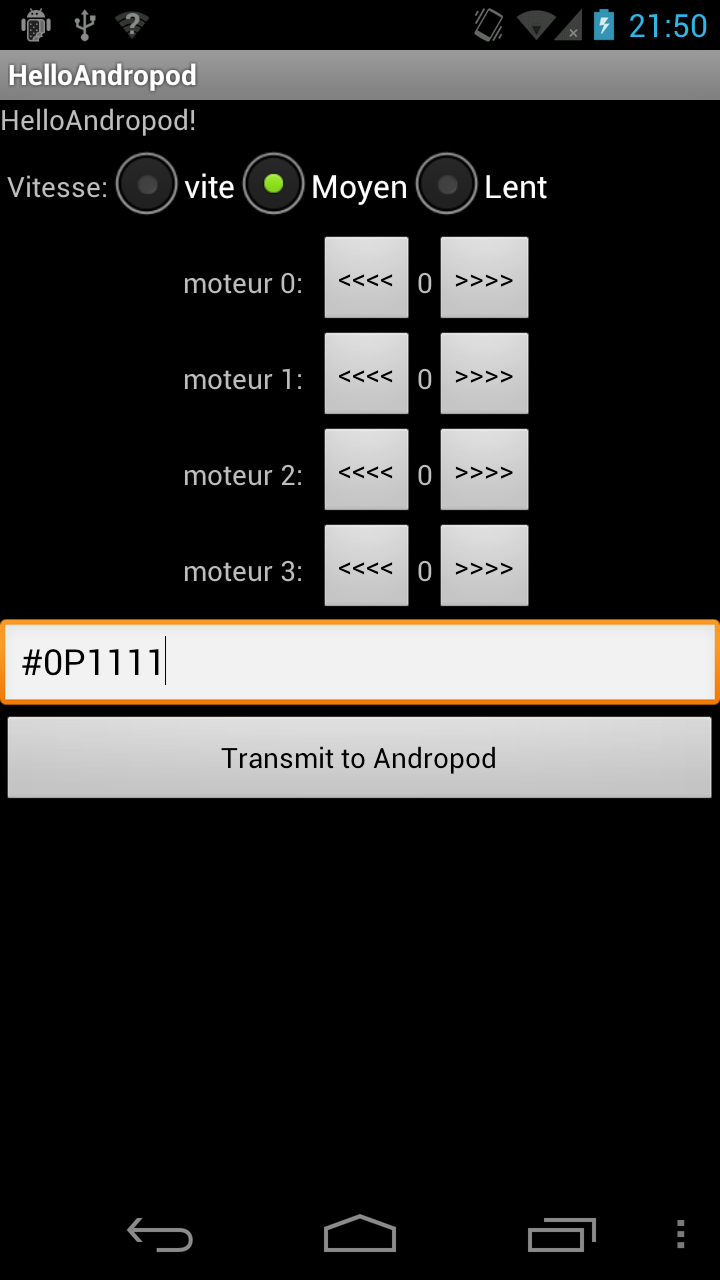
\includegraphics[width=6cm]{pics/ch4_interface.png}%
\caption{L'interface de l'application}%
\label{fig:ch4_interface}%
\end{figure}
%\\[\intextsep]
%\begin{minipage}{\textwidth}
%\centering
%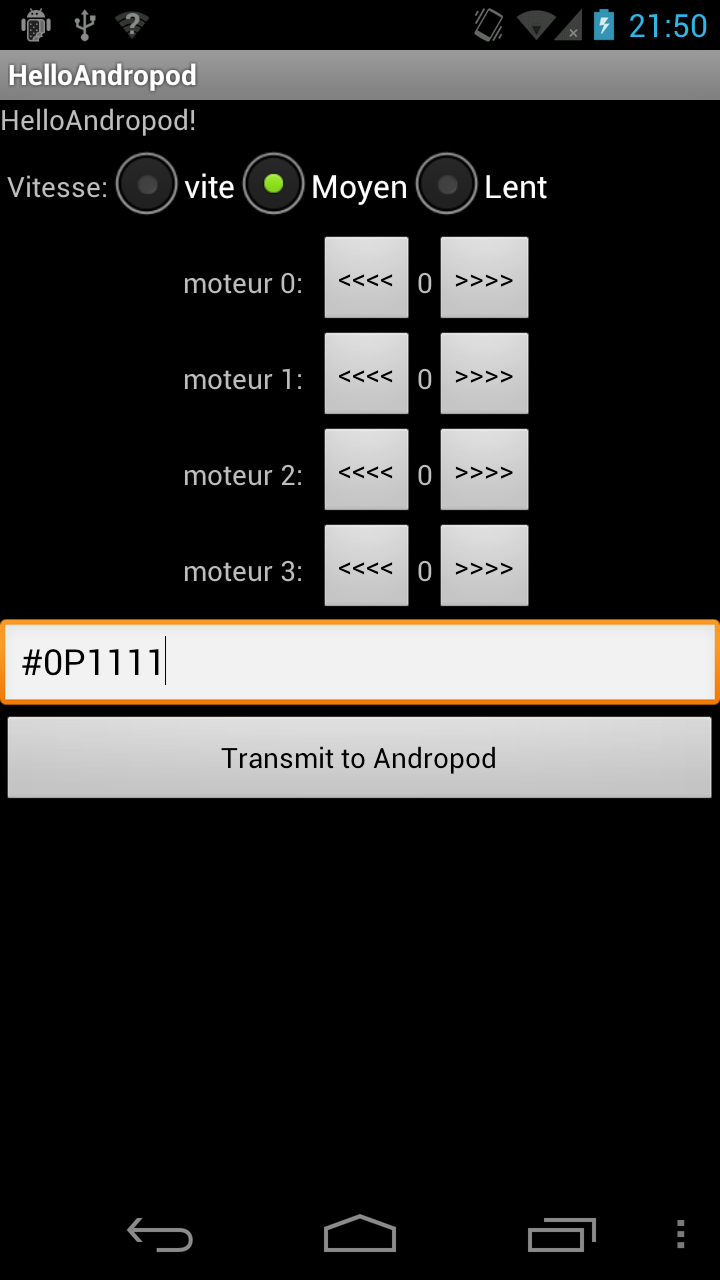
\includegraphics[width=5cm]{pics/ch4_interface.png}
%\label{fig:ch4_interface}
%\end{minipage}
%\\[\intextsep]

A la fin, nous avons reli� toutes les trois parties --- mobile, AndroPOD et ordinateur, et nous avons r�ussit de contr�ler le robot avec notre mobile.

\begin{figure}[!ht]
\centering
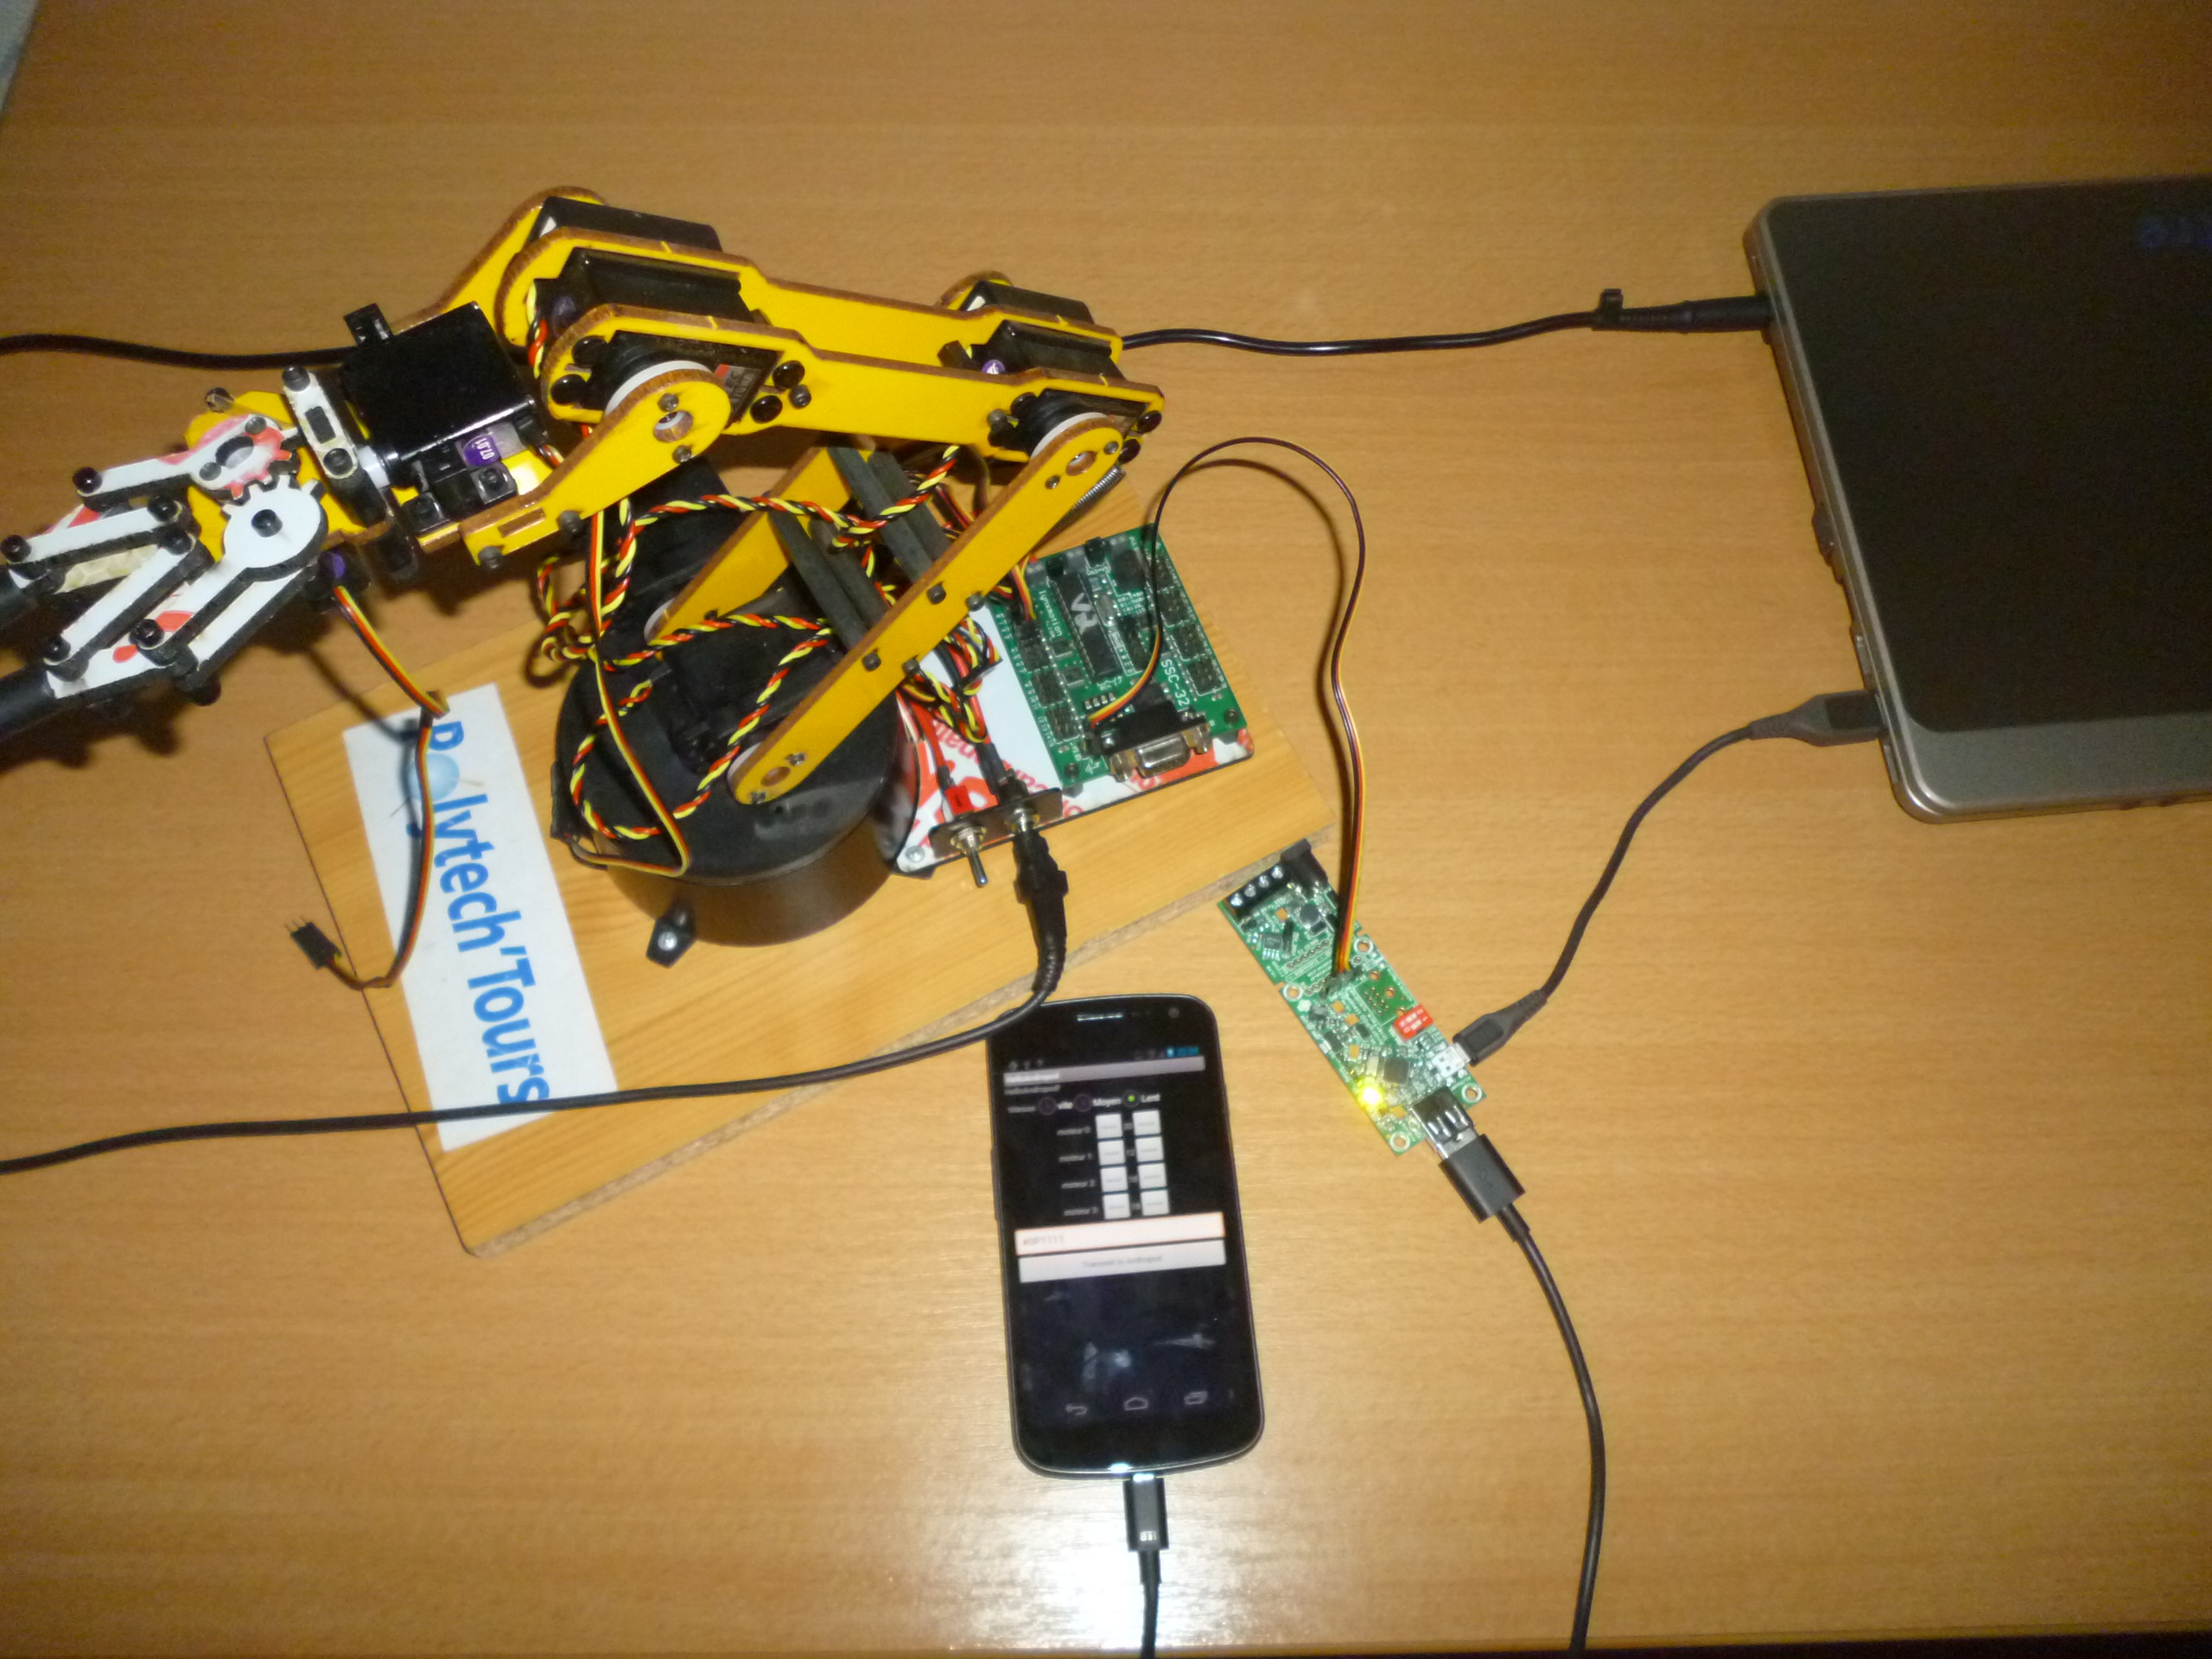
\includegraphics[width=14cm]{pics/ch4_ensemble.JPG}%
\caption{L'oeuvre finale}%
\label{fig:ch4_ensemble}%
\end{figure}